% Created 2021-09-03 Fri 07:32
% Intended LaTeX compiler: pdflatex
\documentclass[11pt]{article}
\usepackage[utf8]{inputenc}
\usepackage[T1]{fontenc}
\usepackage{graphicx}
\usepackage{grffile}
\usepackage{longtable}
\usepackage{wrapfig}
\usepackage{rotating}
\usepackage[normalem]{ulem}
\usepackage{amsmath}
\usepackage{textcomp}
\usepackage{amssymb}
\usepackage{capt-of}
\usepackage{hyperref}
\author{Britt Anderson}
\date{\today}
\title{}
\hypersetup{
 pdfauthor={Britt Anderson},
 pdftitle={},
 pdfkeywords={},
 pdfsubject={},
 pdfcreator={Emacs 27.2 (Org mode 9.4)}, 
 pdflang={English}}
\begin{document}

\tableofcontents

\section{DE Introduction}
\label{sec:org269dba7}

To be able to evaluate lisp in babel blocks you must invoke slime. 
\begin{verbatim}
(format t "~a~%" (list 1 2 3))
\end{verbatim}


\subsection{Can I make a simple plot?}
\label{sec:orge76eb8c}

\subsubsection{First we need a bunch of stuff}
\label{sec:org4cd452a}
\begin{verbatim}
     ;; will need some packages/systems I am sure.
     ;; will try gnuplot -- need to install that package
     ;; and eazy-gnuplot
(ql:quickload '(:eazy-gnuplot :clml.statistics :clml.utility))
(use-package :eazy-gnuplot) 
\end{verbatim}

\subsubsection{Now a basic example?}
\label{sec:org3211d69}
\href{https://guicho271828.github.io/eazy-gnuplot/}{Here} is a "cookbook".

The examples make use of a local subdirectory called "images". Create it.

The first cookbook example seems to use a function we don't need: \texttt{png-from-file}. This is probably related to the cookbook being a jupyter notebook.

\begin{verbatim}
(defun function-plot (output)
  (with-plots (*standard-output* :debug nil)
    (gp-setup :terminal '(pngcairo) :output output)
    (func-plot "[-5:5] (sin(1/x) - cos(x))*erfc(x)"))
  output)
(function-plot "images/function-plot.png")
\end{verbatim}

\begin{center}
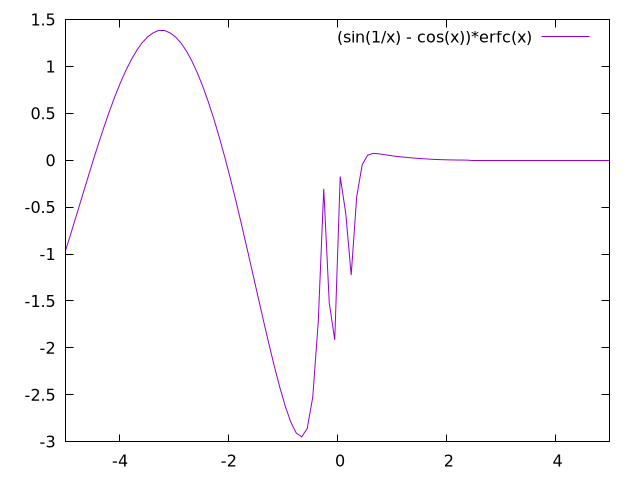
\includegraphics[width=.9\linewidth]{./images/function-plot.png}
\end{center}

\subsubsection{Scatter Plot Example}
\label{sec:org82ec54b}
\begin{verbatim}
(defun scatter-plot (output)
  (let ((point-n 400)
	(point-type 7)
	(point-color "orange"))
    (with-plots (*standard-output* :debug nil)
      (gp-setup :terminal '(pngcairo) :output output)
      (plot
       (lambda ()
	 (loop for p in (map 'list (lambda (x y) (list x y))
			   (clml.statistics:rand-n
			    (clml.statistics:chi-square-distribution 100) point-n)
			   (clml.statistics:rand-n
			    (clml.statistics:chi-square-distribution 10) point-n))
	     do (format t "~&~{~a~^ ~}" p)))
       :with `(:points :pt ,point-type :lc :rgb ,point-color)))
  output))
 (scatter-plot "./images/scatter-plot.png")
\end{verbatim}

\begin{center}
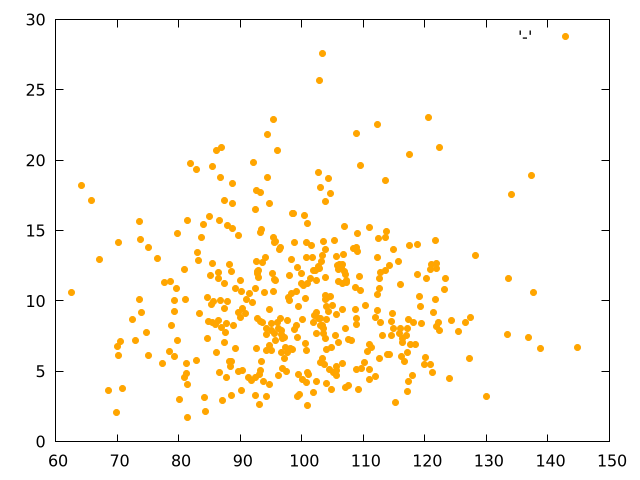
\includegraphics[width=.9\linewidth]{./images/scatter-plot.png}
\end{center}
\end{document}